% -*-cap2.tex-*-
% Este fichero es parte de la plantilla LaTeX para
% la realización de Proyectos Final de Carrera, protegido
% bajo los términos de la licencia GFDL.
% Para más información, la licencia completa viene incluida en el
% fichero fdl-1.3.tex

% Copyright (C) 2009 Pablo Recio Quijano 

\section{Pruebas}

La fase de prueba es de las más importantes de un proyecto software~\cite{art}. El objetivo de este paso es, como razón
última, la verificación de que el proyecto cumple con todos los requisitos iniciales que se plantearon al comienzo 
del desarrollo. Según la metodología clásica de desarrollo de pruebas existen diferentes enfoques a la hora de realizar
este tipo de pruebas de software, siendo todos complementarios~\cite{beizer_software_1990}, pero para el caso
concreto que tenemos entre manos debemos tener en cuenta la naturaleza del proyecto. \\

Los videojuegos presentan dos facetas distintas que deben ser abordadas de diferentes maneras cuando se realiza la fase
de pruebas:
\begin{itemize}
    \item Por un lado tenemos las pruebas clásicas que se realizan a cualquier desarrollo de software, como pueden
            ser las pruebas unitarias o de integración, destinadas a verificar el correcto funcionamiento del
            código.
    \item Y por otro lado, al requerir de una interacción directa con el usuario (y estar destinado a divertir,
            entretener y proporcionar un rato ameno al mismo) se deben realizar varios tipos de pruebas orientadas
            a comprobar que se cumplen requisitos más abstractos como puede ser el testeo o análisis de la jugabilidad
            o usabilidad de la aplicación, interfaces, medir el entretenimiento que proporciona la aplicación (relacionado
            directamente con el desarrollo de la inteligencia artificial de los contrincantes, entre otros)
\end{itemize}

El primer conjunto de pruebas se pueden realizar con comprobaciones de código, compilación (o en este caso concreto,
interpretación) del mismo y diferentes métodos, pero el segundo conjunto de pruebas es necesario que se desarrollen
con diferentes tipos de usuarios reales manejando la aplicación y realizando cuestionarios que nos ayuden a valorar
el éxito o fracaso de estos apartados. \\

Para los apartados de pruebas unitarias y de integración se va a trabajar principalmente con los tres módulos que
forman el núcleo fuerte de la aplicación (y sobre las que cae el peso de la misma):

\begin{itemize}
    \item Sistema de gestión de partida de dominó
    \item Sistema de inteligencia artificial
    \item Motor gráfico de la aplicación
\end{itemize}

\subsection{Pruebas unitarias}

Durante la fase de implementación se fueron realizando pruebas unitarias no automatizadas de cada conjunto o subconjunto
de módulos que se iban desarrollando, evitando así encontrar errores en las pruebas de integración que no sean propiamente
de integración sino de errores en la codificación de los diferentes módulos. \\

Una herramienta cuyo uso ha resultado muy interesante y útil ha sido \textbf{PyFlakes}. Esta herramienta es un programa que
analiza otros programas escritos en Python y detecta un gran conjunto de errores analizando el código fuente. Existen otras
herramientas de análisis automático de código Python, como PyChecker o PyLint, pero se decidió utilizar PyFlakes
principalmente por la rapidez de análisis y seguridad ante caídas, ya que no requiere ejecutar el código, sino que realiza
un análisis mediante \emph{parseo} del código. \\

En cuanto a los diferentes módulos que conforman Dominous, existen varios casos inherentes a cada módulo que deben
tratarse de forma individual (ya que dependen de la naturaleza del módulo) y de forma manual (ya que no se puede abordar su
solución de forma automática).

\subsubsection{Sistema de gestión de partida de dominó}

En este módulo las pruebas unitarias están claras: el módulo debe velar por el correcto cumplimiento de todas y cada
una de las reglas del dominó internacional. Para ello debe vigilarse cada movimiento de los jugadores, repasando
el estado del juego y las diferentes posibilidades que tiene el jugador, entrándose en modo error cuando se realiza
una acción ilegal. \\

En este momento del desarrollo se tuvo que tomar una decisión respecto a cómo contemplar los errores o incumplimiento de
normas que puedan producirse (de forma intencionada o no) por parte de los jugadores:

\begin{itemize}
    \item Una opción era permitir que los jugadores incumplan las normas y actuar en consecuencia contra el jugador.
            En ningún momento se puede permitir que los jugadores coloquen fichas en lugares donde está prohibido
            ese movimiento, por lo que, de todas las normas que posee el dominó las únicas candidatas a entrar en este
            grupo son las que hacen del dominó un \textbf{juego de señores}, es decir, todas aquellas que están destinadas
            a dotar de información a los demás jugadores de forma obligatoria (como puede ser la falta de un palo mediante
            acortar el tiempo que transcurre en su turno).

            Para esta opción teníamos nuevamente otras dos opciones:
            \begin{itemize}
                \item Podemos permitir y \emph{mirar hacia otro lado}, permitiendo que los jugadores engañen de forma
                        clara a los demás jugadores, incluyendo compañeros, o
                \item Podemos actuar como jueces y penalizar a los jugadores que cometan este tipo de faltas.
            \end{itemize}
    \item La otra opción es no permitir este tipo de acciones, volviendo hacia atrás en la acción del jugador y
            pidiendo de nuevo que actúe, hasta que la acción satisfaga las reglas del juego del dominó.
\end{itemize}

Finalmente se decidió que, dado que esta aplicación tiene como requisito el favorecer el aprendizaje del juego del dominó,
no existe cabida alguna a jugadas deshonrosas o que puedan llevar a equivocación al usuario que desea aprender a jugar. \\

Por lo tanto, cuando un jugador intenta realizar una acción equivocada, se deshace esa acción y se le pide de nuevo que
mueva ficha hasta que ese movimiento sea correcto, momento en el cual se continúa con naturalidad la partida.


\subsubsection{Sistema de Inteligencia Artificial}

El juego del dominó es un juego con un amplio universo de acciones y con conocimiento limitado de la situación de la partida,
por lo que no se puede estimar que una acción sea óptima (puede haber varias opciones válidas). Pero a pesar de esto sí existe
un requisito que debe cumplirse (y se exige el cumplimiento) a la hora de realizar un movimiento, y es o pasar o colocar una
ficha cualquiera que pueda colocarse. \\

Esta acción se definió y se tomó como opción por defecto (también llamado fallback) en caso de que todas las demás reglas
de Inetligencia Artificial no se cumplan, y antes de que el sistema quede colgado o no se pueda continuar, se toma esta acción y se continúa
con la partida.


\subsection{Pruebas de integración}

Según se iban desarrollando módulos y éstos cumplían las pruebas unitarias desarrolladas para estos apartados, era necesario
integrar los diferentes módulos para corroborar y contrastar el correcto funcionamiento de la conjunción de ambos módulos.

\begin{figure}[h]
  \begin{center}
    
\includegraphics[scale=1.3]{pruebas_integracion.png}
  \end{center}
  \caption{Esquema de relaciones entre módulos para las pruebas de integración}
  \label{pruebas_integracion}
\end{figure}

\subsubsection{Sistema de Gestión de Partida de Dominó y Sistema de Inteligencia Artificial}

Una vez definida la interfaz de comunicación entre el Sistema de Gestión de Partida de Dominó y Sistema de Inteligencia
Artificial, para comprobar la consistencia de esta integración se desarrolló un jugador de dominó muy simple que debía
cumplir con dos premisas:

\begin{enumerate}
    \item El jugador debe cumplir con éxito las especificaciones de la interfaz.
    \item El jugador debe poner una ficha cualquiera (si puede colocar una ficha) o debe pasar (si no existe la posibilidad
            de mover).
\end{enumerate}

Durante el desarrollo del Sistema de Gestión de Partida de Dominó se fue comprobando el éxito de la comunicación entre ambos
módulos, de tal modo que cuando se realizó la integración con los dos sistemas totalmente finalizados no se encontraron
problemas graves, obteniéndose una integración suave y sin errores costosos de solventar.

\subsubsection{Sistema de Gestión de Partida de Dominó y Motor gráfico de la aplicación}

La integración fue más costosa que la comentada anteriormente, ya que no se pudo realizar un sistema de pruebas que
cumpliera las especificaciones de integración, pero gracias a que el Sistema de Gestión de Partida de Dominó contaba
con un gran número de métodos de todo tipo para obtener información del estado del tablero, jugadores y otros,
se pudo realizar la integración de forma sencilla y sin retrasarnos en demasía en la estimación de tiempos.


\subsection{Pruebas de Jugabilidad, usabilidad y experiencia de usuario}

La jugabilidad en Dominous abarca dos ámbitos diferenciados: por un lado se desea que el juego transcurra fluido, sin
parones bruscos o bajadas en la velocidad de cálculo y dibujado de la pantalla, y por otro lado que el jugador, al mover
fichas y desenvolverse por el juego y los menús. \\

El desempeño o velocidad de la aplicación está asegurado por varios factores:

\begin{itemize}
    \item Utilización de una biblioteca de bajo nivel como es PyGame, cuya velocidad está garantizada y testeada en profundidad.
    \item La naturaleza propia de la aplicación, que se desarrolla a un ritmo bajo, no necesita de grandes cálculos ni
            uso avanzado de la CPU.
    \item El motor de inteligencia artificial es rápido, y en casos en los que las posibilidades del usuario se limiten
            a pasar o colocar una única ficha, el motor salta todas las comprobaciones de reglas que sabe que van a
            fallar --- redundando así en una mayor velocidad y rendimiento.
\end{itemize}

\begin{figure}[h]
  \begin{center}
    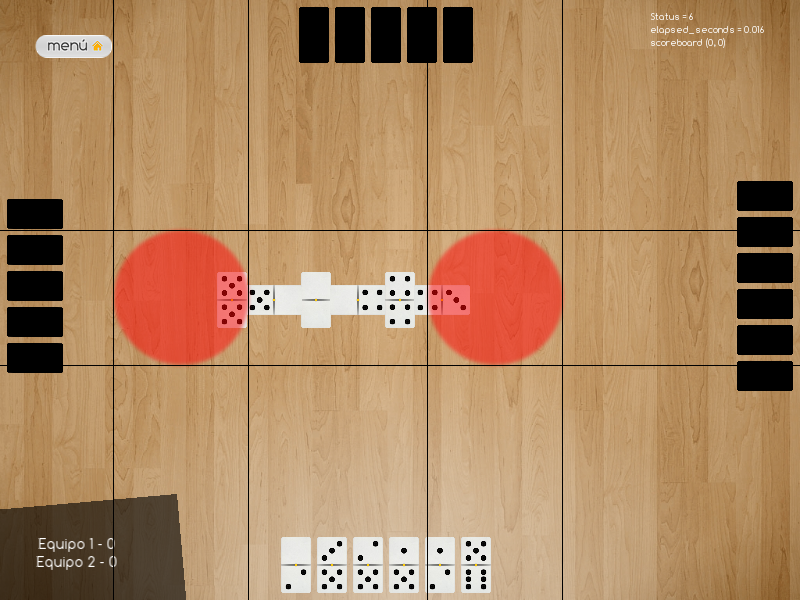
\includegraphics[scale=0.8]{superficie_drop.png}
  \end{center}
  \caption{Superficie sobre la cual el usuario puede dejar la ficha satisfactoriamente}
  \label{superficie_drop}
\end{figure}


La jugabilidad de la aplicación, dado que la acción más común que realizará el usuario será mover las fichas,
se trabajó haciendo que el movimiento de arrastrar y soltar la ficha sea satisfactorio, cuidando que la ficha siga
al cursor de forma fiel, el error de soltar una ficha en un lugar equivocado no sea frustrante --- sino que se convierta
en un hecho más de la partida ---, que la zona donde el usuario suelta la ficha sea grande y no se produzcan errores
no deseados y funcionalidades y pequeñas mejoras que buscan que el jugador se divierta con la aplicación. \\

\begin{figure}[h]
  \begin{center}
    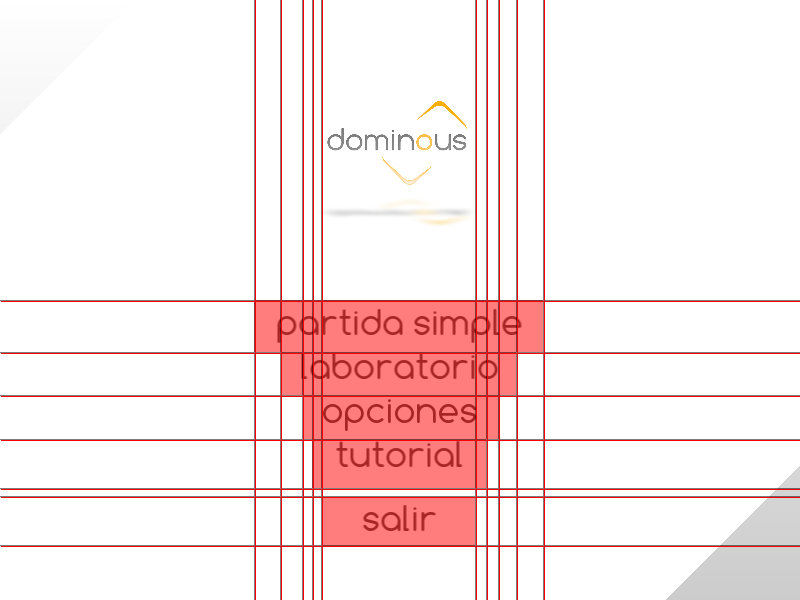
\includegraphics[scale=0.8]{superficie_click.png}
  \end{center}
  \caption{Como vemos, la superficie en la cual el usuario puede realizar click de forma satisfactoria es más amplia que el simple texto que incluye}
  \label{superficie_click}
\end{figure}

Dado que la aplicación está orientado a un público adulto --- que, probablemente, no goce de una habilidad muy desarrollada
con los dispositivos de entrada --- la zona de click sobre menús y demás elementos de la interfaz se ha agrandado, con lo
cual las posibilidades de éxito del click aumentan, así como la satisfacción del usuario con la herramienta. \\

Por último, se han realizado numerosas pruebas con usuarios reales durante el desarrollo del proyecto, recibiendo
feedback real y realizando y estudiando pequeñas modificaciones que hagan que el mismo disfrute de la experiencia de
jugar a este producto. \\

Los usuarios sobre los que se han realizado las diferentes pruebas son los siguientes:

\begin{description}
    \item[Sujeto 1] Mujer, 28 años, estudios universitarios de la rama de letras, nivel de informática usuario alto, con conocimientos
        de ofimática, poca experiencia en videojuegos, bajo nivel de las reglas y normas del dominó internacional.
    \item[Sujeto 2] Hombre, 63 años, estudios universitarios de economía, nivel de informática usuario medio, nula experiencia en
        videojuegos, jugador experimentado de dominó.
    \item[Sujeto 3] Hombre, 30 años, estudios universitarios de Informática, alto nivel de informática usuario, amplia experiencia
        en videojuegos, nivel medio de conocimiento del juego de dominó.
    \item[Sujeto 4] Hombre, 31 años, estudios universitarios de Informática, alto nivel de informática usuario, amplia experiencia
        en videojuegos, nivel bajo de conocimiento del juego de dominó.

\end{description}

Se analizó el uso de la aplicación por parte de los sujetos con las siguientes circunstancias:

\begin{itemize}
    \item Todas las pruebas se realizaron en un ordenador portátil con ratón, ejecutándose la aplicación en un entorno Windows 7.
    \item Se les proporcionó la aplicación ya en ejecución, mostrándoles la pantalla de inicio.
    \item No se les facilitó ningún tipo de información adicional sobre cómo funciona la aplicación.
\end{itemize}

Por otra parte, los objetivos a cumplir eran los siguientes:

\begin{description}
    \item[Objetivo 1] Comenzar una partida simple, jugar una mano, salir al menú principal y cerrar la aplicación.
    \item[Objetivo 2] Cambiar el tema gráfico, seleccionando el tema \textbf{fruits} comenzar una partida simple,
            jugar una mano, salir al menú principal y cerrar la aplicación.
    \item[Objetivo 3] Seleccionar el modo \textbf{solo computadora} en velocidad rápida, visualizar una mano, salir
            al menú principal y cerrar la aplicación.
    \item[Objetivo 4] Entrar en \textbf{laboratorio}, hacer que compitan dos equipos diferentes y comentar con el
            entrevistador cuál de los dos equipos ha conseguido más victorias.
\end{description}

Y los éxitos de objetivos y resultados obtenidos se detallan a continuación:

\begin{description}
    \item[Objetivo 1] Todos los sujetos fueron capaces de completar con éxito el objetivo 1. Cabe destacar que los sujetos
            tres y cuatro salieron al menú principal activando el menú de juego con la tecla \textbf{escape}, y el
            sujeto cuatro salió de la aplicación cerrando directamente la ventana de la misma, sin hacer uso del
            botón salir que se encuentra en el menú principal de Dominous.
    \item[Objetivo 2] Todos los sujetos fueron capaces de completar con éxito el objetivo 2, aunque el usuario dos
            necesitó de información acerca de qué es un tema gráfico --- la información se le proporcionó debido a que el
            bajo nivel de conocimiento informático no permitía el éxito de este objetivo.
    \item[Objetivo 3] Todos los sujetos fueron capaces de completar con éxito este objetivo, pero se produjeron los
            siguientes hechos meritorios de ser comentados:
            \begin{itemize}
                \item El usuario dos se sintió desconcertado cuando se iban produciendo los movimientos automáticos
                    de los jugadores, y preguntó que qué utilidad podía tener ver una partida a esta velocidad y sin
                    participar.
                \item El usuario uno de frustró y preguntó cómo podía salir de la aplicación, a pesar de que la interfaz
                    para volver al menú principal era la misma que en el modo de juego simple.
            \end{itemize}
    \item[Objetivo 4] Los usuarios uno, tres y cuatro completaron con éxito este objetivo. El usuario dos no fue
            capaz de comprender el significado de la gráfica o de las barras, y no entendió el uso que podía tener el
            enfrentar a dos equipos si no puedes ver el transcurso de las partidas.
\end{description}
